\documentclass[12pt,a4paper]{article}
\usepackage{graphicx}
\usepackage{amsmath}
\usepackage{amssymb}

\title{\textbf{BÁO CÁO BÀI TẬP LỚN}\\ Môn: Học sâu\\ Xấp xỉ hàm mật độ Gaussian hai chiều bằng mạng perceptron đa tầng}
\author{Sinh viên thực hiện: Dương Tấn Cường\\ Mã số sinh viên: 3123580004}
\date{Tháng 10 năm 2026}

\begin{document}

\maketitle

\section*{Tóm tắt}

Báo cáo trình bày việc xây dựng và huấn luyện mạng perceptron đa tầng (MLP) để xấp xỉ hàm mật độ Gaussian hai chiều trên miền $x_1 \in [-2, 2]$, $x_2 \in [-4, 4]$, với $\boldsymbol{\mu} = (0, 0)$ và ma trận hiệp phương sai $C = \begin{bmatrix}0.3 & -0.5\\ -0.5 & 2\end{bmatrix}$. Toàn bộ mô hình được cài đặt bằng PyTorch thuần với \texttt{torch.nn.Module}, \texttt{nn.Linear}, \texttt{TensorDataset}/\texttt{DataLoader}, \texttt{MSELoss} và bộ tối ưu Adam; vòng lặp huấn luyện được viết thủ công gồm forward, tính loss, xóa gradient, lan truyền ngược và cập nhật tham số. Dữ liệu được sinh ngẫu nhiên với seed cố định, chia thành 2000 mẫu train, 1000 mẫu validation và 100 mẫu test độc lập.

Ba nhóm thực nghiệm có kiểm soát được tiến hành: (A) ảnh hưởng của số mẫu huấn luyện từ 200 đến 2000; (B) ảnh hưởng của số nơ-ron tầng ẩn từ 1 đến 10 với một tầng ẩn; (C) ảnh hưởng của số tầng ẩn từ 1 đến 4. Mỗi cấu hình được chạy với ba seed và báo cáo trung bình cùng độ lệch chuẩn. Kết quả cho thấy sai số giảm khoảng 19 lần khi tăng số mẫu từ 200 lên 2000, giảm khoảng 42 lần khi tăng độ rộng từ 1 lên 10 nơ-ron, và chỉ cải thiện khoảng 2.8 lần khi tăng độ sâu từ 1 lên 4 tầng. Mô hình cuối cùng được chọn theo validation loss và đạt MSE $1.09\times10^{-6}$, MAE $7.97\times10^{-4}$ trên tập test 100 mẫu.

\section{1. Giới thiệu}

\subsection{1.1. Bối cảnh và mục tiêu}

Mạng nơ-ron nhiều tầng là một trong những công cụ mạnh nhất để xấp xỉ các hàm phi tuyến liên tục. Với bài toán hai chiều, một mạng MLP nhỏ vẫn có thể đạt sai số rất thấp nếu dữ liệu được lấy mẫu đủ dày và quá trình huấn luyện được kiểm soát tốt. Tuy nhiên, chất lượng xấp xỉ không chỉ phụ thuộc vào kiến trúc mà còn vào số lượng mẫu, cách chia dữ liệu và cách chọn mô hình. Việc chỉ báo cáo một cấu hình duy nhất thường không đủ để hiểu hành vi của mạng.

Mục tiêu của bài tập lớn này gồm bốn điểm: (i) cài đặt đúng công thức hàm mật độ Gaussian hai chiều và quy trình sinh dữ liệu có thể tái lập; (ii) thiết kế MLP tùy biến số tầng và số nơ-ron bằng PyTorch, tự viết vòng lặp huấn luyện và validation; (iii) thực hiện ba nhóm thực nghiệm có kiểm soát về quy mô dữ liệu, độ rộng và độ sâu; (iv) đánh giá định lượng, trực quan hóa kết quả và rút ra nhận xét có căn cứ thay vì chỉ trình bày hình ảnh.

\subsection{1.2. Phát biểu bài toán}

Cho hàm mật độ Gaussian hai chiều
$$f(\mathbf{x}) = \frac{1}{2\pi\sqrt{\det(C)}} \exp\left[-\frac{1}{2}(\mathbf{x}-\boldsymbol{\mu})^T C^{-1}(\mathbf{x}-\boldsymbol{\mu})\right],$$
với
$$\boldsymbol{\mu} = \begin{bmatrix}0\\0\end{bmatrix}, \qquad C = \begin{bmatrix}0.3 & -0.5\\ -0.5 & 2\end{bmatrix}.$$
Cần xây dựng mạng MLP nhận đầu vào $\mathbf{x} = (x_1, x_2)$ và cho đầu ra $\hat{y}$ sao cho $\hat{y} \approx f(\mathbf{x})$ trên miền $-2 \le x_1 \le 2$ và $-4 \le x_2 \le 4$. Dữ liệu huấn luyện được sinh ngẫu nhiên theo phân bố đều trên miền khảo sát, nhãn là giá trị hàm thật không kèm nhiễu. Tập test gồm 100 mẫu độc lập; ngoài ra có một tập validation riêng phục vụ chọn mô hình.

\subsection{1.3. Đóng góp và bố cục}

Báo cáo có ba đóng góp chính. Thứ nhất, mã nguồn được tổ chức thành các khối chức năng rõ ràng (sinh dữ liệu, định nghĩa mô hình, huấn luyện, đánh giá, chạy thực nghiệm) và có thể chạy lại từ đầu. Thứ hai, ba thực nghiệm A/B/C được thiết kế để chỉ thay đổi một yếu tố tại một thời điểm, nhờ đó có thể quy kết xu hướng sai số cho yếu tố đang khảo sát. Thứ ba, mọi kết quả đều đi kèm log CSV, hình và checkpoint, giúp kiểm chứng số liệu trong báo cáo.

Phần còn lại được tổ chức như sau. Mục 2 trình bày dữ liệu và cách chia tập. Mục 3 mô tả kiến trúc MLP, hàm mất mát và quy trình huấn luyện. Mục 4 trình bày ba nhóm thực nghiệm cùng kết quả định lượng. Mục 5 thảo luận các xu hướng, trường hợp bất thường và hạn chế. Mục 6 kết luận.

\section{2. Dữ liệu}

\subsection{2.1. Công thức và tham số}

Với tham số đã cho, định thức và hệ số chuẩn hóa của hàm mật độ là
$$\det(C) = 0.3\cdot 2 - (-0.5)(-0.5) = 0.35, \qquad \frac{1}{2\pi\sqrt{\det(C)}} = 3.717183.$$
Ma trận nghịch đảo là
$$C^{-1} = \frac{1}{0.35}\begin{bmatrix}2 & 0.5\\ 0.5 & 0.3\end{bmatrix} \approx \begin{bmatrix}5.7143 & 1.4286\\ 1.4286 & 0.8571\end{bmatrix}.$$
Giá trị đỉnh của hàm tại tâm là $f(0,0) = 1/(2\pi\sqrt{0.35}) \approx 0.269021$. Việc kiểm tra tích phân số trên một lưới rộng cho kết quả xấp xỉ $1.0000$, xác nhận công thức và hằng số chuẩn hóa được cài đặt đúng.

Hàm có hiệp phương sai âm giữa hai biến nên các đường đồng mức nghiêng theo hướng tương quan nghịch: khi $x_1$ tăng thì $x_2$ có xu hướng giảm. Đây là đặc điểm quan trọng mà mô hình cần học; một mạng quá hẹp hoặc chỉ có một tầng ẩn nhỏ sẽ khó biểu diễn đồng thời độ nhọn của đỉnh và hướng nghiêng này.

\subsection{2.2. Lấy mẫu và chia dữ liệu}

Dữ liệu được sinh bằng cách lấy mẫu đều trên miền khảo sát:
$$x_1 \sim \mathcal{U}[-2, 2], \qquad x_2 \sim \mathcal{U}[-4, 4], \qquad y = f(x_1, x_2).$$
Ba tập được sinh từ ba seed khác nhau để bảo đảm độc lập:

\begin{itemize}
\item \textbf{Master train pool:} 2000 mẫu, seed $43$.
\item \textbf{Validation:} 1000 mẫu, seed $44$.
\item \textbf{Test:} 100 mẫu, seed $45$.
\end{itemize}

Trong thực nghiệm A, tập con huấn luyện được lấy lồng nhau theo thứ tự \texttt{pool[:A]}. Cách làm này bảo đảm mọi cấu hình $A$ đều dùng chung một phân bố dữ liệu và các tập nhỏ là tập con của tập lớn, tránh nhiễu do sinh lại dữ liệu. Validation và test giữ nguyên tuyệt đối trong mọi lần chạy. Seed khởi tạo mạng và seed xáo trộn dữ liệu của ba lần lặp là 42, 43 và 44.

Tập test chỉ được dùng để báo cáo kết quả cuối; không dùng để chọn siêu tham số hay dừng sớm. Validation được dùng cho checkpoint, early stopping và lựa chọn mô hình. Việc phân tách vai trò này được giữ nhất quán trong toàn bộ báo cáo.

\subsection{2.3. Thống kê và trực quan hóa}

Bảng 1 tóm tắt thống kê mô tả của master train pool. Hai biến vào phân bố gần như đều và đối xứng quanh 0, đúng như cách lấy mẫu. Ngược lại, $y$ lệch phải mạnh: trung bình chỉ khoảng $0.0291$ nhưng đỉnh đạt $0.2681$, và có tới $63.1\%$ số mẫu có $y < 0.01$. Phần lớn mẫu nằm ở vùng đuôi mật độ thấp, trong khi vùng đỉnh chỉ chiếm một tỷ lệ nhỏ.

\begin{table}[h]
\centering
\caption{Bảng 1. Thống kê mô tả master train pool (2000 mẫu).}
\begin{tabular}{|c|c|c|c|c|}
\hline
Biến & Trung bình & Độ lệch chuẩn & Nhỏ nhất & Lớn nhất \\
\hline
$x_1$ & 0.0223 & 1.1646 & $-1.9911$ & 1.9982 \\
\hline
$x_2$ & $-0.0592$ & 2.3473 & $-3.9900$ & 3.9991 \\
\hline
$y$ & 0.0291 & 0.0543 & $0.0000$ & 0.2681 \\
\hline
\end{tabular}
\end{table}

Hình 1 minh họa 700 mẫu train ngẫu nhiên, bề mặt hàm thật và đường đồng mức mật độ. Hình 2 cho thấy phân bố của từng biến: $x_1$ và $x_2$ gần như phẳng, còn $y$ tập trung sát 0 với một đuôi kéo dài về phía giá trị lớn. Sự mất cân bằng này có hệ quả trực tiếp đến huấn luyện: mô hình có thể đạt MSE nhỏ bằng cách dự đoán gần 0 ở hầu hết điểm, nhưng khi đó vùng đỉnh sẽ bị xấp xỉ kém. Vì vậy, ngoài MSE cần theo dõi MAE, RMSE và trực quan hóa $y$–$\hat{y}$ cùng bề mặt xấp xỉ.

\begin{figure}[h]
\centering
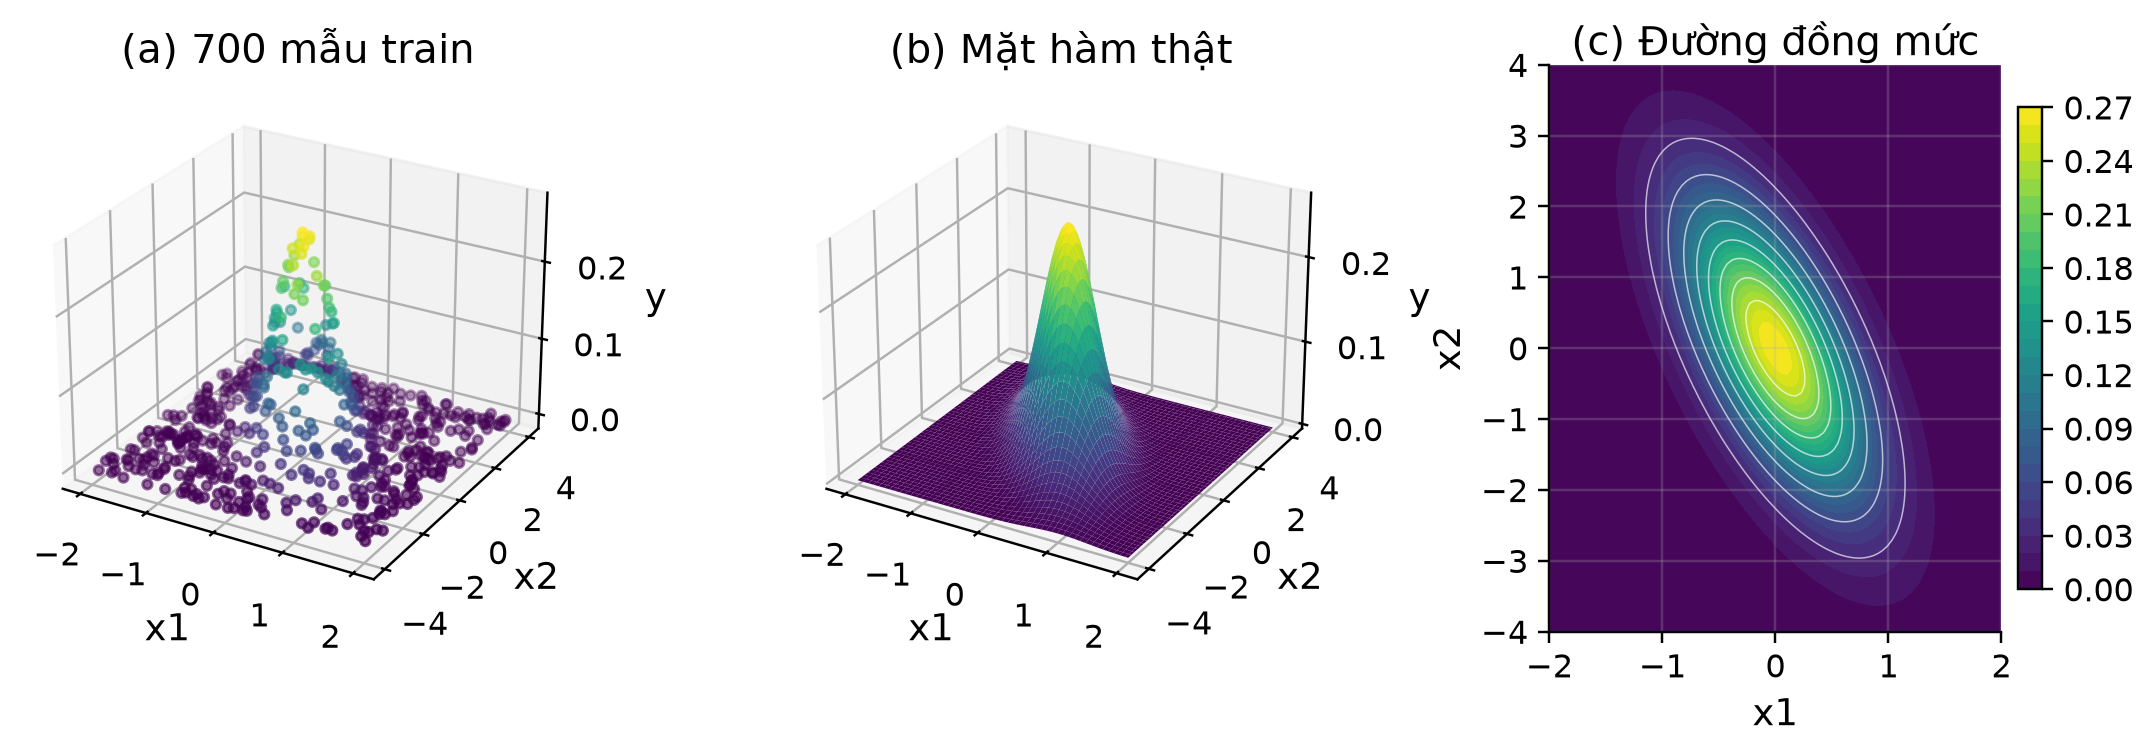
\includegraphics[width=1.0\textwidth]{figures/r01_data_overview.png}
\caption{Hình 1. Dữ liệu Gaussian 2D: (a) 700 mẫu train ngẫu nhiên; (b) bề mặt hàm thật; (c) đường đồng mức mật độ trên miền khảo sát.}
\end{figure}

\begin{figure}[h]
\centering
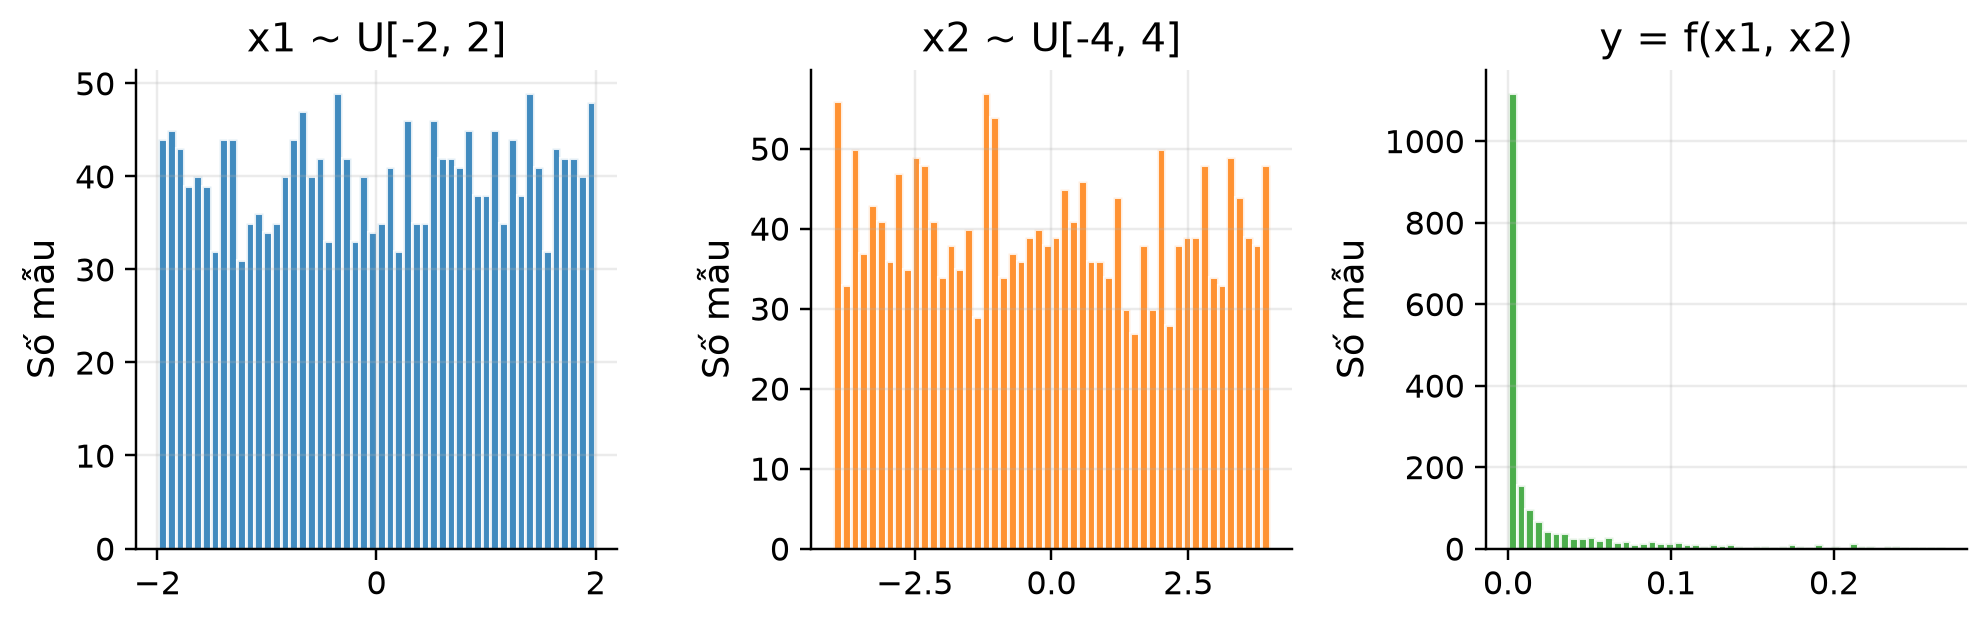
\includegraphics[width=1.0\textwidth]{figures/r02_data_distributions.png}
\caption{Hình 2. Phân bố $x_1$, $x_2$ và $y$ trên master train pool. $x_1$, $x_2$ gần như đều; $y$ lệch phải mạnh và tập trung sát 0.}
\end{figure}

\subsection{2.4. Nhận xét về dữ liệu}

Có ba điểm cần lưu ý. Thứ nhất, hàm mục tiêu trơn và không có nhiễu, nên sai số quan sát được chủ yếu phản ánh năng lực xấp xỉ và mức độ che phủ của dữ liệu, không bị chi phối bởi nhiễu đo. Thứ hai, do $y$ tập trung ở vùng nhỏ, MSE tuyệt đối rất thấp ngay cả khi mô hình chưa học tốt vùng đỉnh; cần đối chiếu thêm MAE và hình $y$–$\hat{y}$. Thứ ba, tương quan mẫu giữa $x_1$ và $x_2$ gần 0 ($r \approx 0.010$) vì dữ liệu được lấy đều trên hình chữ nhật; tương quan âm của hàm mục tiêu nằm trong $C$, không nằm trong phân bố lấy mẫu. Điều này có nghĩa mô hình phải học tương quan từ nhãn chứ không thể suy ra từ phân bố đầu vào.

\section{3. Mô hình và cài đặt}

\subsection{3.1. Kiến trúc MLP}

Mạng nhận vector hai chiều $\mathbf{x} = (x_1, x_2)$, đi qua $C$ tầng ẩn với $B$ nơ-ron mỗi tầng, rồi cho một đầu ra vô hướng. Với tầng ẩn thứ $l$:
$$\mathbf{h}^{(l)} = \sigma\left(W^{(l)}\mathbf{h}^{(l-1)} + \mathbf{b}^{(l)}\right), \qquad l = 1, \ldots, C,$$
và đầu ra
$$\hat{y} = W^{(C+1)}\mathbf{h}^{(C)} + b^{(C+1)}.$$
Hàm kích hoạt mặc định là $\tanh$, được chọn vì đạo hàm trơn và phù hợp với bài toán hồi quy có đầu ra nhỏ, liên tục. Lớp ra tuyến tính không kích hoạt để mô hình có thể biểu diễn giá trị dương trong khoảng $[0, 0.27]$.

Kiến trúc được cài đặt bằng một lớp con của \texttt{torch.nn.Module}. Số tầng và số nơ-ron là tham số khởi tạo, cho phép tái sử dụng cùng một lớp cho cả ba thực nghiệm. Với cấu hình baseline hai tầng ẩn 64 nơ-ron, số tham số huấn luyện là 4417: $2\cdot64+64 = 192$ tham số ở tầng đầu, $64\cdot64+64 = 4160$ ở tầng thứ hai và $64\cdot1+1 = 65$ ở lớp ra.

\subsection{3.2. Hàm mất mát và bộ tối ưu}

Mô hình được huấn luyện bằng MSE:
$$\mathcal{L}(\theta) = \frac{1}{N}\sum_{i=1}^{N}\left(\hat{y}_i - y_i\right)^2,$$
trong đó $N$ là số mẫu của lô. MSE phù hợp với bài toán hồi quy và có đạo hàm đơn giản, thuận lợi cho lan truyền ngược. Bộ tối ưu Adam được dùng với learning rate $5\times10^{-3}$; đây là lựa chọn phổ biến cho mạng nhỏ vì hội tụ nhanh và ít nhạy với việc chọn learning rate ban đầu.

Ngoài MSE, báo cáo dùng MAE và RMSE để đánh giá:
$$\mathrm{MAE} = \frac{1}{N}\sum_{i=1}^{N}\left|\hat{y}_i - y_i\right|, \qquad \mathrm{RMSE} = \sqrt{\frac{1}{N}\sum_{i=1}^{N}\left(\hat{y}_i - y_i\right)^2}.$$
MAE có đơn vị của $y$ và ít bị chi phối bởi các sai số lớn ở vùng đỉnh; RMSE nhấn mạnh sai số lớn. Sử dụng đồng thời ba chỉ số giúp tránh kết luận phiến diện.

\subsection{3.3. Vòng lặp huấn luyện và validation}

Mỗi epoch gồm hai pha. Trong pha huấn luyện, mô hình được đặt ở chế độ \texttt{train()}, dữ liệu được duyệt theo từng batch và thực hiện tuần tự: tính đầu ra, tính loss, xóa gradient cũ, lan truyền ngược và cập nhật tham số. Trong pha validation, mô hình chuyển sang \texttt{eval()}, tắt tính gradient bằng \texttt{torch.no_grad()} và tính MSE trên tập validation. Trọng số tốt nhất theo validation loss được lưu lại; nếu sau 50 epoch liên tiếp không cải thiện quá $10^{-7}$, quá trình huấn luyện dừng sớm.

Cấu hình huấn luyện baseline được tóm tắt trong Bảng 2. Các thực nghiệm A/B/C chỉ thay đổi đúng biến khảo sát, giữ nguyên các siêu tham số còn lại.

\begin{table}[h]
\centering
\caption{Bảng 2. Cấu hình huấn luyện baseline.}
\begin{tabular}{|c|c|}
\hline
Tham số & Giá trị \\
\hline
Số mẫu huấn luyện $A$ & 1000 \\
\hline
Kiến trúc & 2 tầng ẩn, 64 nơ-ron/tầng \\
\hline
Hàm kích hoạt & $\tanh$ \\
\hline
Bộ tối ưu & Adam \\
\hline
Learning rate & $5\times10^{-3}$ \\
\hline
Batch size & 64 \\
\hline
Số epoch tối đa & 300 \\
\hline
Early stopping & patience 50, min delta $10^{-7}$ \\
\hline
Thiết bị & CPU \\
\hline
\end{tabular}
\end{table}

\subsection{3.4. Môi trường và tổ chức mã nguồn}

Mã nguồn được cài đặt bằng Python với PyTorch, NumPy, Pandas và Matplotlib. Dữ liệu được bọc trong \texttt{TensorDataset} và \texttt{DataLoader}; mỗi lần chạy tạo một generator riêng với seed cố định để thứ tự xáo trộn có thể tái lập. Checkpoint của từng lượt chạy được lưu dưới dạng \texttt{.pt}, kèm cấu hình kiến trúc, seed, validation loss tốt nhất và số epoch đã chạy. Kết quả và lịch sử loss được ghi ra CSV.

Môi trường tham chiếu: Python 3.12, PyTorch 2.14.0 (CPU), NumPy 2.5.3, Pandas 3.0.5, Matplotlib 3.11.2. Toàn bộ thí nghiệm chạy trên CPU; không sử dụng GPU. Mã nguồn không phụ thuộc đường dẫn tuyệt đối, các thư mục đầu ra được tạo tự động khi chạy.

\section{4. Thực nghiệm}

\subsection{4.1. Quy trình đánh giá công bằng}

Mỗi cấu hình được chạy với ba seed 42, 43, 44. Với mỗi seed, mô hình được khởi tạo lại và thứ tự dữ liệu được xáo trộn lại, nhưng dữ liệu train/validation/test và kiến trúc giữ nguyên. Kết quả báo cáo là trung bình và độ lệch chuẩn trên ba lần chạy, trừ baseline và mô hình cuối được báo cáo riêng như mô tả ở các mục tương ứng.

Ba nguyên tắc được tuân thủ. Thứ nhất, chỉ một yếu tố được thay đổi trong mỗi nhóm thực nghiệm. Thứ hai, tập test không tham gia vào bất kỳ quyết định nào về kiến trúc, learning rate hay early stopping. Thứ ba, mọi lượt chạy đều được lưu log và checkpoint để có thể kiểm chứng lại số liệu. Các bảng test trong mục 4.3--4.5 nhằm mục đích báo cáo và so sánh, không dùng để chọn mô hình; việc chọn mô hình cuối chỉ dựa trên validation loss.

\subsection{4.2. Kết quả baseline}

Baseline dùng 1000 mẫu train, kiến trúc 2×64 và các siêu tham số trong Bảng 2. Quá trình huấn luyện dừng sớm ở epoch 196; trọng số tốt nhất đạt được ở epoch 146 với validation MSE $2.98\times10^{-6}$. Bảng 3 trình bày sai số trên ba tập.

\begin{table}[h]
\centering
\caption{Bảng 3. Kết quả baseline trên train, validation và test.}
\begin{tabular}{|c|c|c|c|}
\hline
Tập & MSE & MAE & RMSE \\
\hline
Train (1000 mẫu) & $3.13\times10^{-6}$ & $1.42\times10^{-3}$ & $1.77\times10^{-3}$ \\
\hline
Validation (1000 mẫu) & $2.98\times10^{-6}$ & $1.39\times10^{-3}$ & $1.73\times10^{-3}$ \\
\hline
Test (100 mẫu) & $3.26\times10^{-6}$ & $1.37\times10^{-3}$ & $1.80\times10^{-3}$ \\
\hline
\end{tabular}
\end{table}

Sai số test rất nhỏ so với đỉnh hàm $f(0,0) \approx 0.269$: MAE chỉ khoảng $0.5\%$ giá trị đỉnh. Ba giá trị train, validation và test gần như trùng nhau, cho thấy không có dấu hiệu quá khớp. Đường loss trong Hình 3 giảm nhanh trong khoảng 30--50 epoch đầu rồi bão hòa; validation loss còn dao động nhẹ ở mức $10^{-6}$ nhưng không tăng, nên early stopping chủ yếu tiết kiệm thời gian hơn là chống quá khớp.

\begin{figure}[h]
\centering
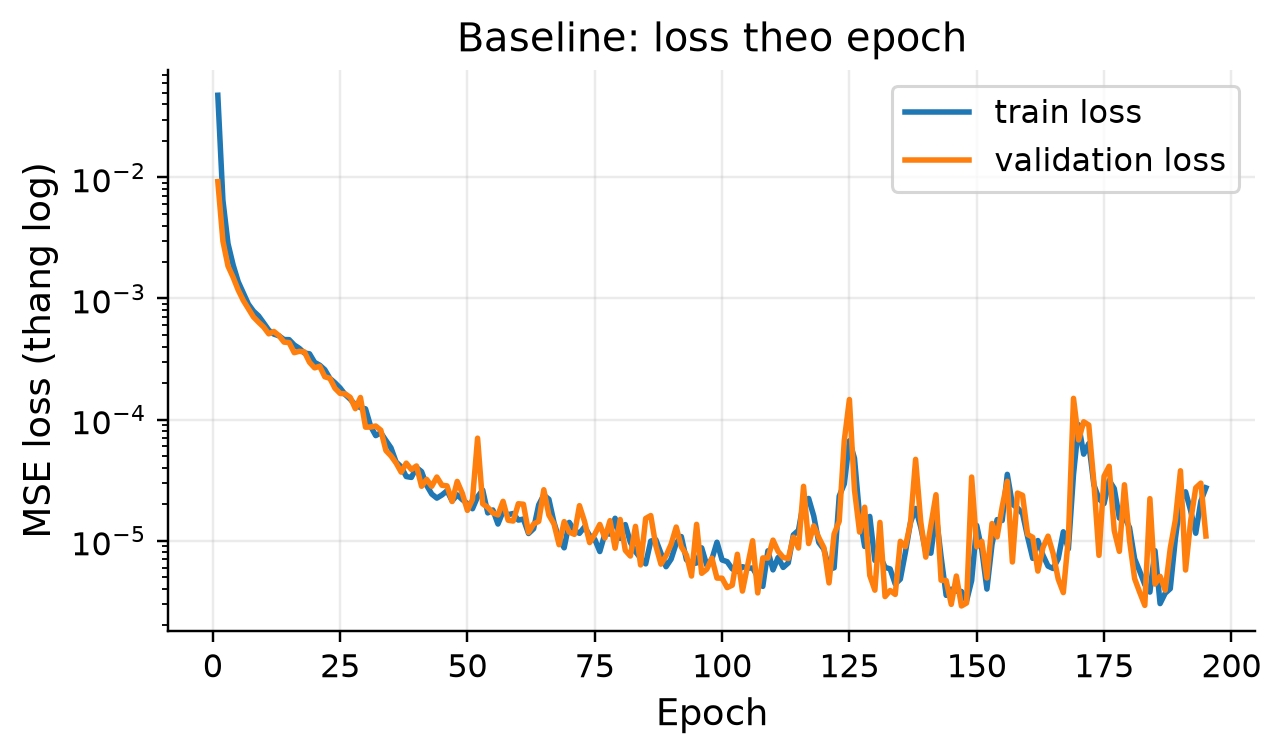
\includegraphics[width=0.75\textwidth]{figures/r03_baseline_loss.png}
\caption{Hình 3. Đường loss train và validation của baseline theo epoch (thang log).}
\end{figure}

Hình 4 so sánh $y$ thật và $\hat{y}$ trên 100 mẫu test; các điểm bám sát đường $y = \hat{y}$, kể cả ở vùng đỉnh. Hình 5 cho thấy bề mặt xấp xỉ tái tạo đúng hình dạng và hướng nghiêng của bề mặt thật. Đây là mốc so sánh cho các thực nghiệm tiếp theo.

\begin{figure}[h]
\centering
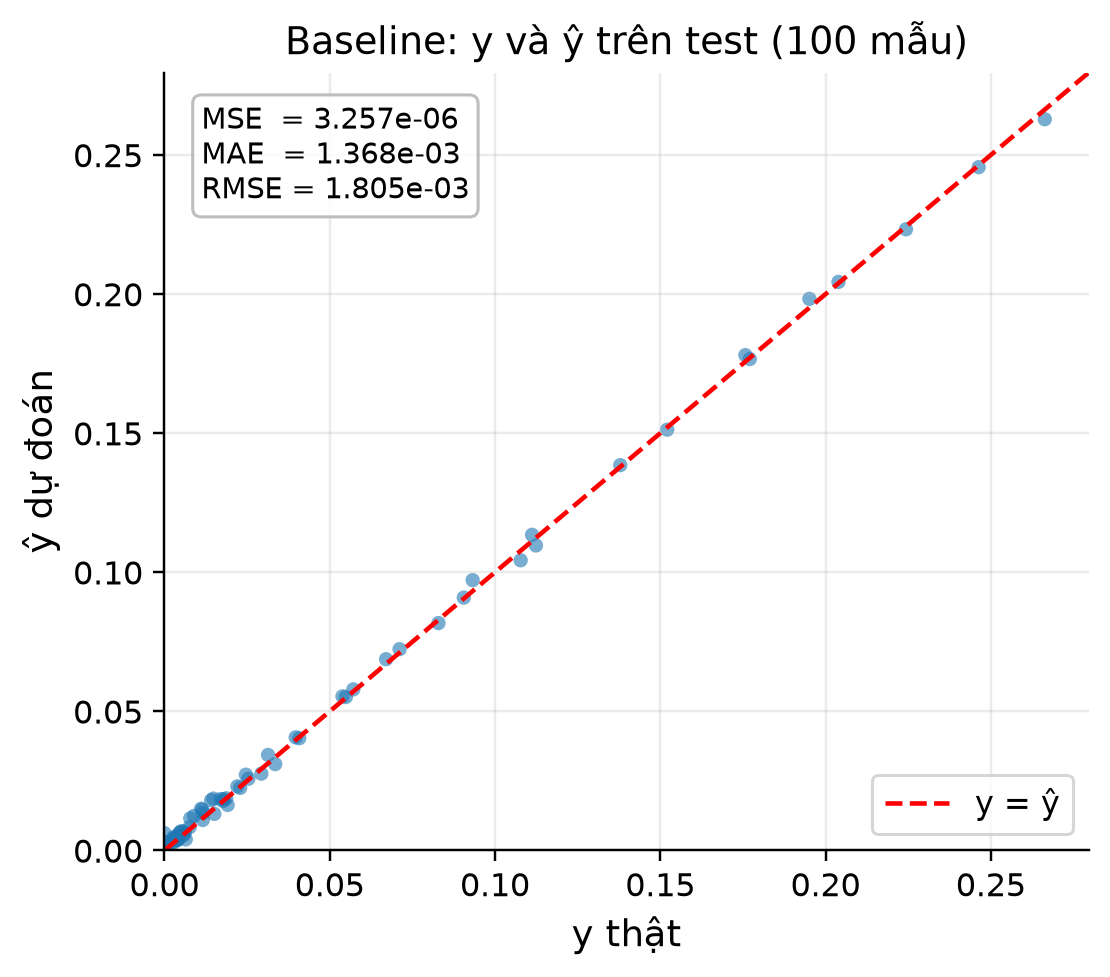
\includegraphics[width=0.62\textwidth]{figures/r04_baseline_yhat.png}
\caption{Hình 4. Baseline: so sánh $y$ thật và $\hat{y}$ trên tập test (100 mẫu).}
\end{figure}

\begin{figure}[h]
\centering
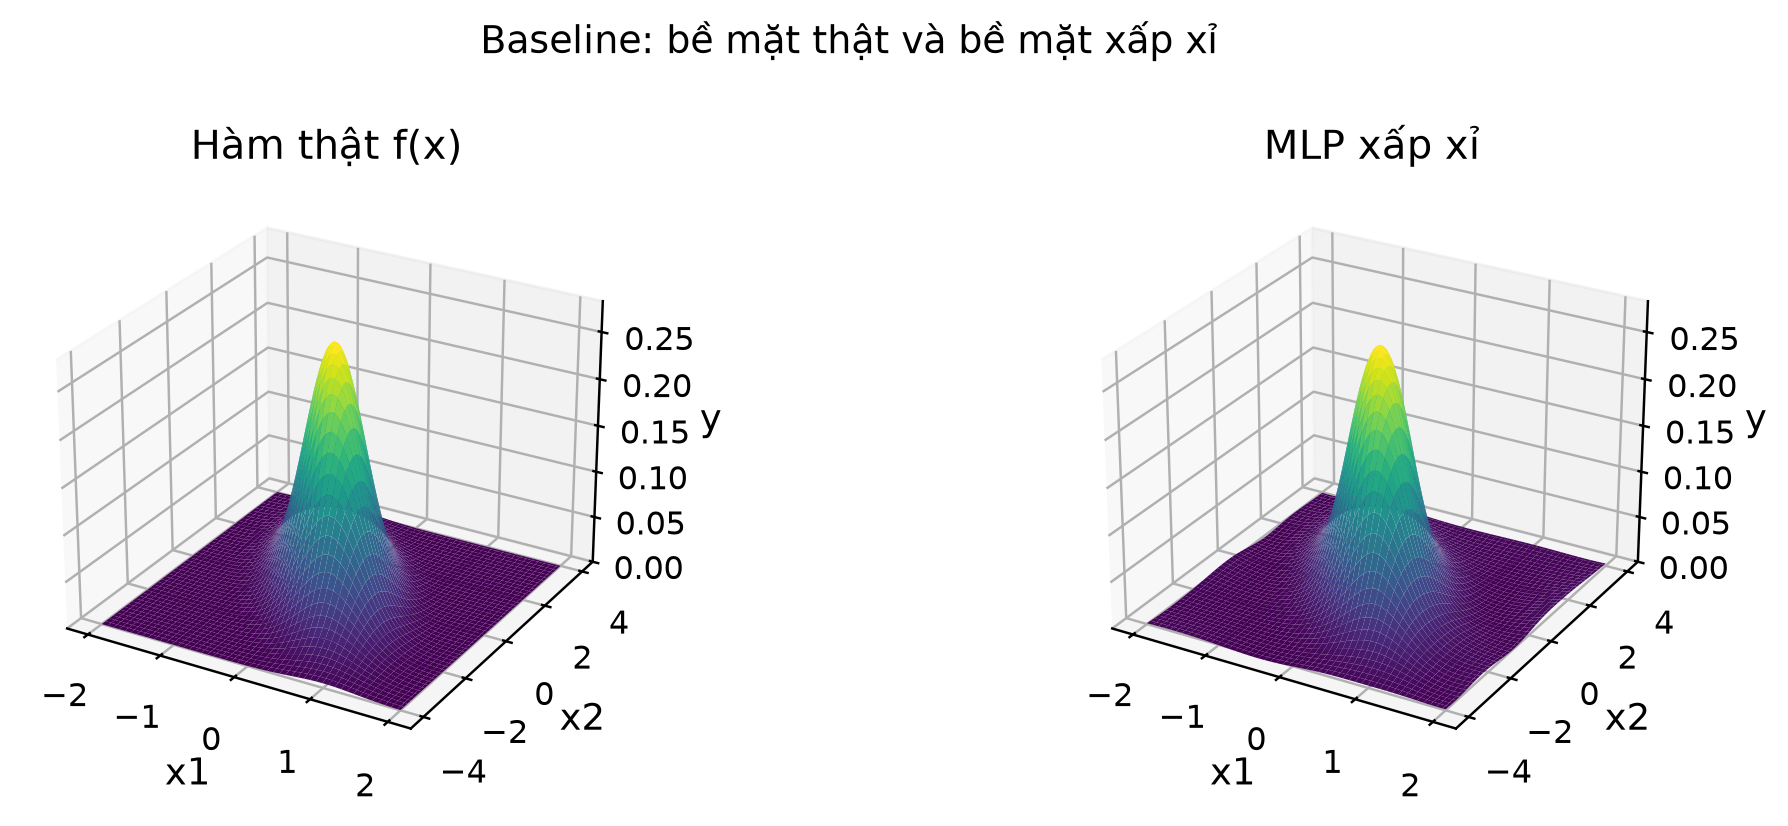
\includegraphics[width=0.95\textwidth]{figures/r05_baseline_surface.png}
\caption{Hình 5. Baseline: so sánh bề mặt hàm thật và bề mặt xấp xỉ của MLP.}
\end{figure}

\subsection{4.3. Thực nghiệm A: ảnh hưởng của số mẫu huấn luyện}

Thực nghiệm A thay đổi số mẫu huấn luyện $A \in \{200, 400, \ldots, 2000\}$ và giữ nguyên kiến trúc 2×64. Bảng 4 báo cáo sai số test trung bình và độ lệch chuẩn trên ba seed. Hình 6 biểu diễn cùng dữ liệu dưới dạng đồ thị có thanh sai số; Hình 7 so sánh train, validation và test MSE.

\begin{table}[h]
\centering
\caption{Bảng 4. Thực nghiệm A: sai số test theo số mẫu huấn luyện (trung bình ± độ lệch chuẩn, 3 seed).}
\begin{tabular}{|c|c|c|c|}
\hline
$A$ & Test MSE & Test MAE & Test RMSE \\
\hline
200 & $(2.37 \pm 0.61)\times10^{-5}$ & $3.89\times10^{-3}$ & $4.84\times10^{-3}$ \\
\hline
400 & $(7.11 \pm 2.73)\times10^{-6}$ & $1.99\times10^{-3}$ & $2.63\times10^{-3}$ \\
\hline
600 & $(3.89 \pm 0.32)\times10^{-6}$ & $1.46\times10^{-3}$ & $1.97\times10^{-3}$ \\
\hline
800 & $(2.91 \pm 2.08)\times10^{-6}$ & $1.28\times10^{-3}$ & $1.64\times10^{-3}$ \\
\hline
1000 & $(4.23 \pm 0.92)\times10^{-6}$ & $1.65\times10^{-3}$ & $2.05\times10^{-3}$ \\
\hline
1200 & $(1.29 \pm 0.21)\times10^{-6}$ & $9.18\times10^{-4}$ & $1.13\times10^{-3}$ \\
\hline
1400 & $(1.40 \pm 0.77)\times10^{-6}$ & $9.10\times10^{-4}$ & $1.16\times10^{-3}$ \\
\hline
1600 & $(1.41 \pm 0.54)\times10^{-6}$ & $9.13\times10^{-4}$ & $1.17\times10^{-3}$ \\
\hline
1800 & $(2.06 \pm 0.42)\times10^{-6}$ & $1.09\times10^{-3}$ & $1.43\times10^{-3}$ \\
\hline
2000 & $(1.22 \pm 0.12)\times10^{-6}$ & $8.77\times10^{-4}$ & $1.11\times10^{-3}$ \\
\hline
\end{tabular}
\end{table}

\begin{figure}[h]
\centering
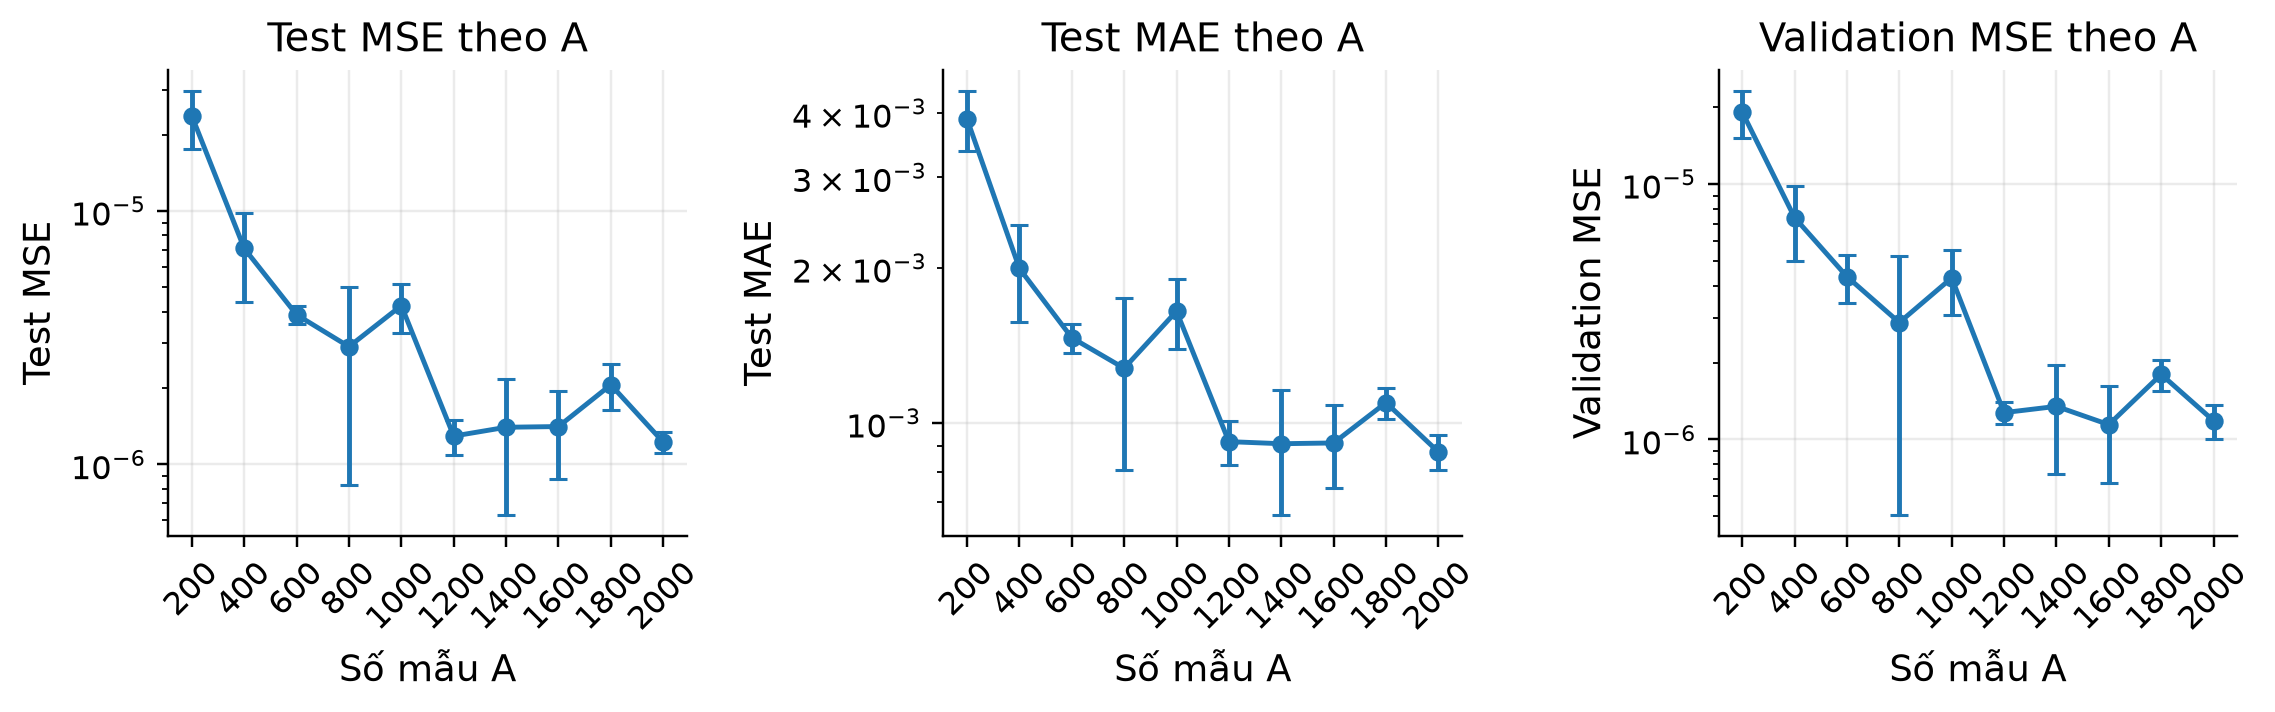
\includegraphics[width=1.0\textwidth]{figures/r06_expA.png}
\caption{Hình 6. Thực nghiệm A: test MSE, test MAE và validation MSE theo số mẫu huấn luyện (mean ± std, 3 seed).}
\end{figure}

\begin{figure}[h]
\centering
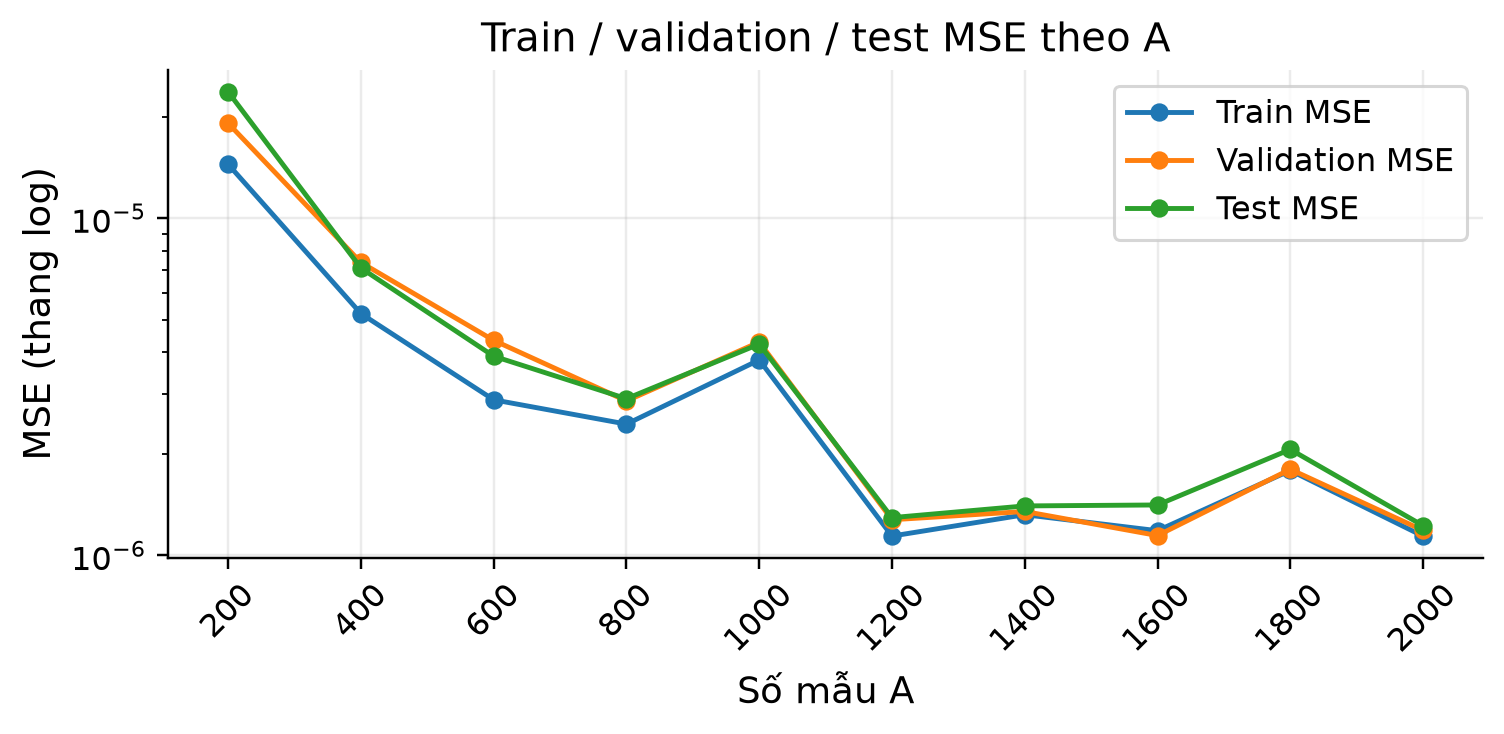
\includegraphics[width=0.8\textwidth]{figures/r07_expA_gap.png}
\caption{Hình 7. Thực nghiệm A: so sánh train, validation và test MSE theo $A$.}
\end{figure}

Sai số giảm mạnh khi tăng $A$: test MSE giảm từ $2.37\times10^{-5}$ ở $A=200$ xuống $1.22\times10^{-6}$ ở $A=2000$, tức khoảng 19 lần; MAE giảm từ $3.89\times10^{-3}$ xuống $8.77\times10^{-4}$, khoảng 4.4 lần. Tốc độ cải thiện không đều: giảm nhanh từ $A=200$ đến $600$--$800$, sau đó hiệu suất biên giảm. Từ $A \ge 1200$, test MSE dao động quanh $1$--$2\times10^{-6}$ và không giảm đơn điệu; ví dụ $A=1800$ có sai số cao hơn $A=1600$. Ở thang sai số này, dao động chủ yếu do khởi tạo mạng và thời điểm dừng sớm, không phải do thiếu dữ liệu.

Độ lệch chuẩn giữa ba seed giảm từ $6.1\times10^{-6}$ ở $A=200$ xuống $1.2\times10^{-7}$ ở $A=2000$, cho thấy mô hình ổn định hơn khi có nhiều dữ liệu. Khoảng cách train--validation nhỏ ở mọi $A$; ngay cả $A=200$ cũng chỉ có train MSE $1.44\times10^{-5}$ so với validation $1.91\times10^{-5}$. Với bài toán hai chiều và mạng 2×64, quá khớp không phải vấn đề chính; nút thắt là lượng dữ liệu che phủ vùng đỉnh nhọn. Kết luận, $A \approx 1000$--$1200$ là điểm cân bằng; dùng toàn bộ 2000 mẫu cho mô hình cuối vẫn hợp lý vì cải thiện nhẹ và không gây quá khớp.

\subsection{4.4. Thực nghiệm B: ảnh hưởng của độ rộng tầng ẩn}

Thực nghiệm B khảo sát $B \in \{1, 2, \ldots, 10\}$ nơ-ron trong một tầng ẩn duy nhất ($C=1$), cố định $A=1000$ và các siêu tham số còn lại. Bảng 5 báo cáo sai số test, train và validation; Hình 8 biểu diễn sai số theo $B$, Hình 9 so sánh đường hội tụ validation của một số cấu hình.

\begin{table}[h]
\centering
\caption{Bảng 5. Thực nghiệm B: ảnh hưởng của số nơ-ron tầng ẩn (1 tầng ẩn, 3 seed).}
\begin{tabular}{|c|c|c|c|c|c|}
\hline
$B$ & Tham số & Test MSE & Test MAE & Train MSE & Validation MSE \\
\hline
1 & 5 & $3.46\times10^{-3}$ & $3.82\times10^{-2}$ & $3.01\times10^{-3}$ & $2.84\times10^{-3}$ \\
\hline
2 & 9 & $2.59\times10^{-3}$ & $3.26\times10^{-2}$ & $2.27\times10^{-3}$ & $2.15\times10^{-3}$ \\
\hline
3 & 13 & $2.03\times10^{-3}$ & $2.75\times10^{-2}$ & $1.80\times10^{-3}$ & $1.77\times10^{-3}$ \\
\hline
4 & 17 & $5.96\times10^{-4}$ & $1.73\times10^{-2}$ & $5.52\times10^{-4}$ & $5.66\times10^{-4}$ \\
\hline
5 & 21 & $5.06\times10^{-4}$ & $1.65\times10^{-2}$ & $4.40\times10^{-4}$ & $4.60\times10^{-4}$ \\
\hline
6 & 25 & $3.31\times10^{-4}$ & $1.36\times10^{-2}$ & $3.26\times10^{-4}$ & $3.32\times10^{-4}$ \\
\hline
7 & 29 & $2.35\times10^{-4}$ & $1.17\times10^{-2}$ & $2.09\times10^{-4}$ & $2.05\times10^{-4}$ \\
\hline
8 & 33 & $1.77\times10^{-4}$ & $9.79\times10^{-3}$ & $1.43\times10^{-4}$ & $1.44\times10^{-4}$ \\
\hline
9 & 37 & $8.35\times10^{-5}$ & $6.86\times10^{-3}$ & $7.53\times10^{-5}$ & $8.53\times10^{-5}$ \\
\hline
10 & 41 & $8.20\times10^{-5}$ & $6.75\times10^{-3}$ & $7.42\times10^{-5}$ & $8.35\times10^{-5}$ \\
\hline
\end{tabular}
\end{table}

\begin{figure}[h]
\centering
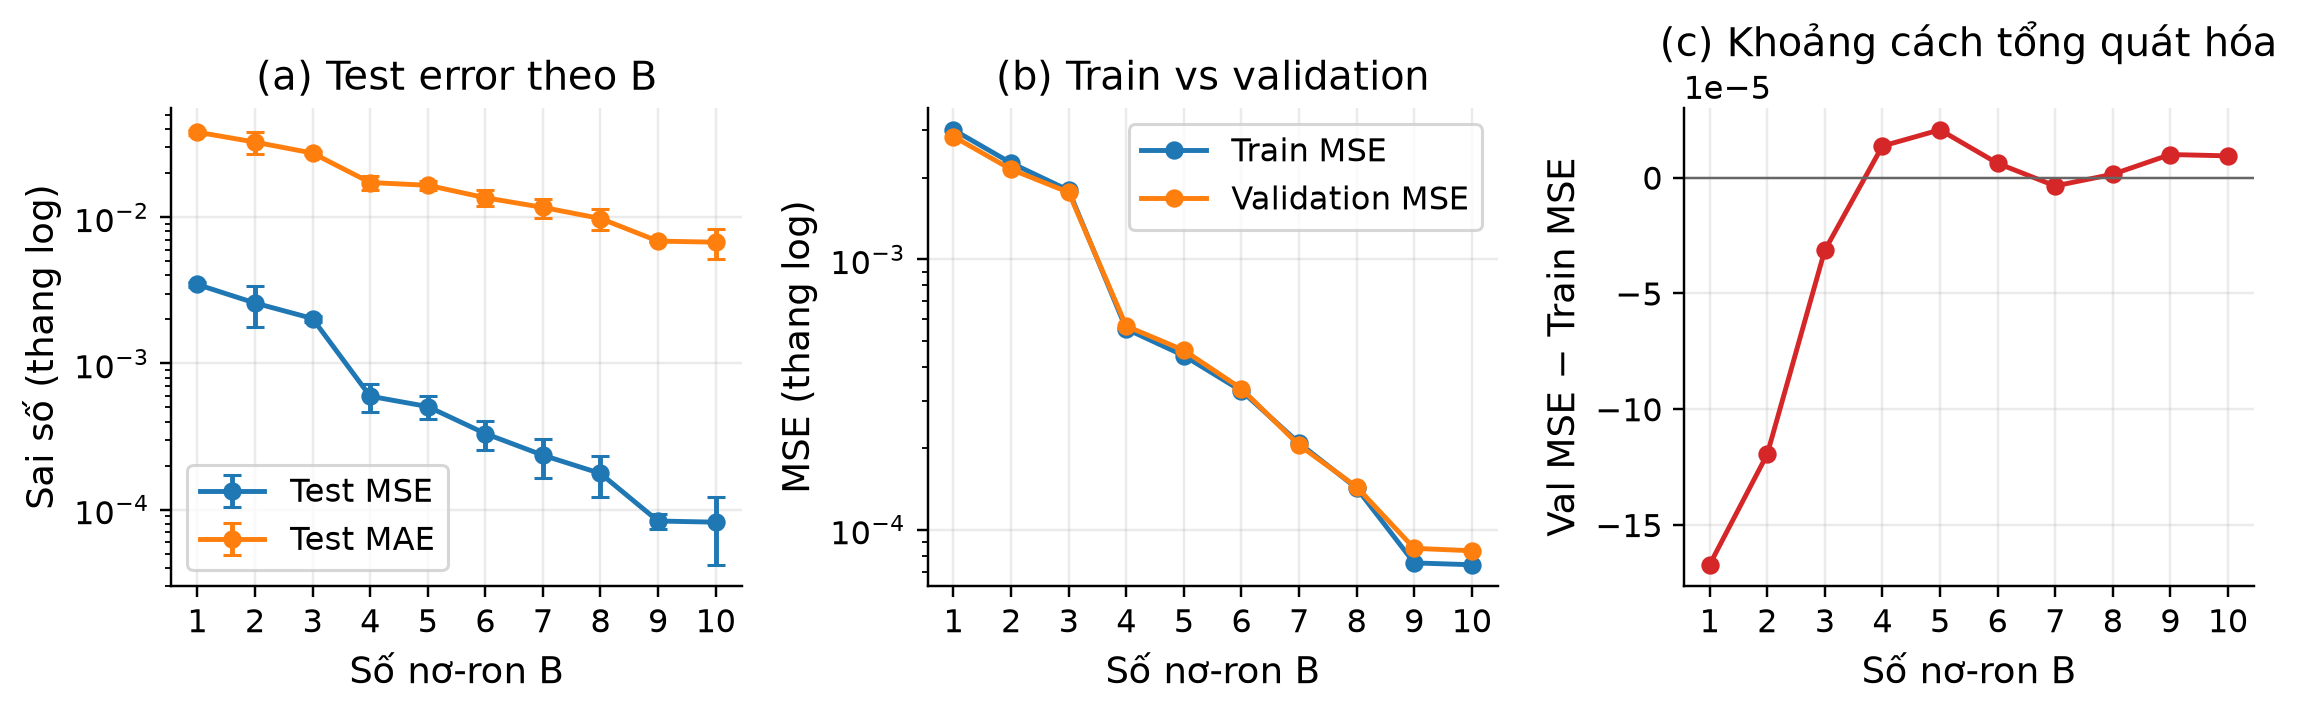
\includegraphics[width=1.0\textwidth]{figures/r08_expB.png}
\caption{Hình 8. Thực nghiệm B: (a) test error theo $B$; (b) train và validation MSE; (c) khoảng cách tổng quát hóa validation -- train.}
\end{figure}

\begin{figure}[h]
\centering
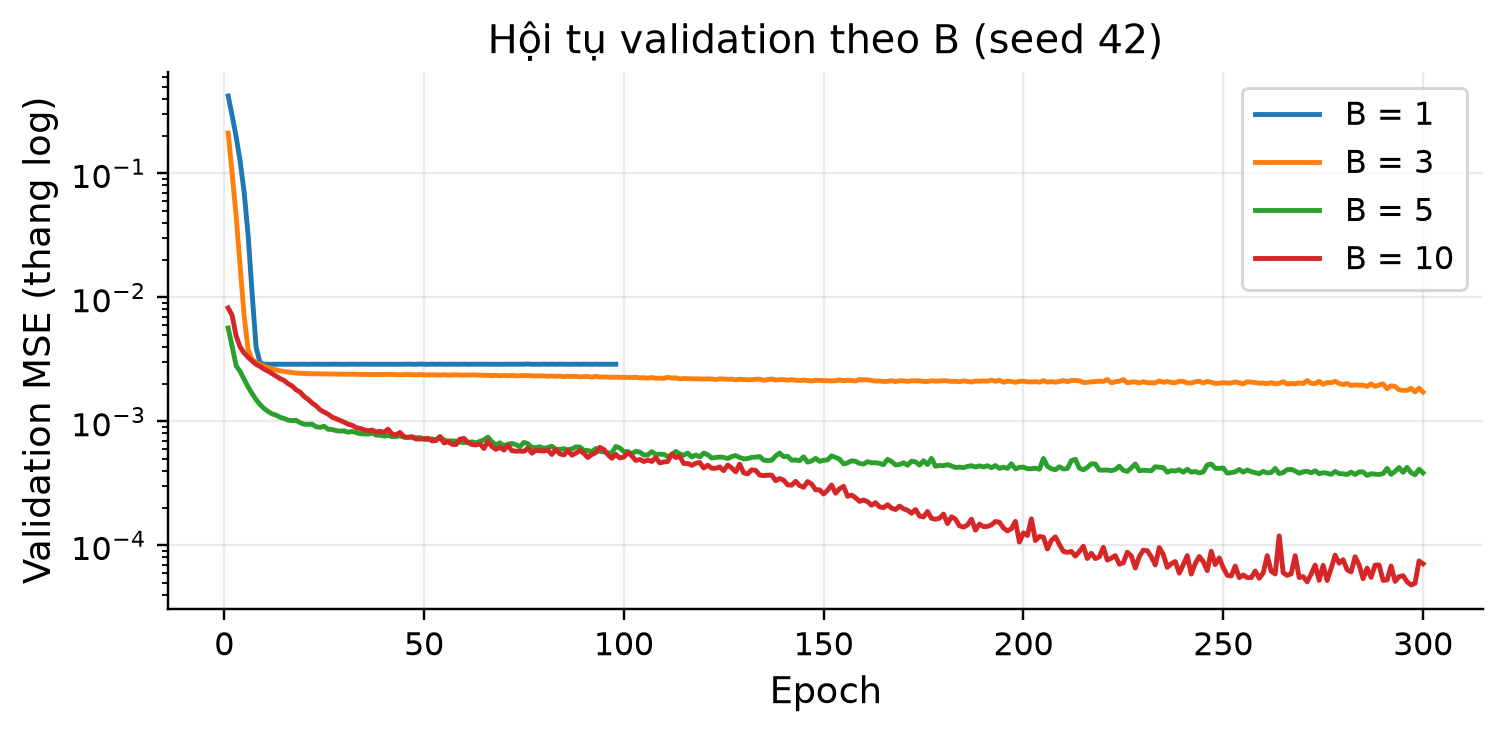
\includegraphics[width=0.8\textwidth]{figures/r09_expB_conv.png}
\caption{Hình 9. Thực nghiệm B: đường hội tụ validation của các cấu hình $B = 1, 3, 5, 10$ (seed 42).}
\end{figure}

Khi $B$ quá nhỏ, mạng thiếu khớp rõ rệt. Với $B=1$, test MSE $3.46\times10^{-3}$ xấp xỉ phương sai của $y$ (khoảng $0.00295$), nghĩa là mạng gần như chỉ dự đoán giá trị trung bình. $B=2$ và $B=3$ vẫn rất kém vì một tầng ẩn quá hẹp không biểu diễn được đỉnh nhọn và tương quan âm. Test MSE giảm đơn điệu khi tăng $B$, từ $3.46\times10^{-3}$ xuống $8.20\times10^{-5}$ (khoảng 42 lần). Bước nhảy lớn nhất nằm giữa $B=3$ và $B=4$ (giảm khoảng 3.4 lần), cho thấy ngưỡng năng lực tối thiểu nằm quanh bốn nơ-ron.

Chưa thấy quá khớp trong dải $B \le 10$: train MSE và validation MSE gần như trùng nhau, chênh lệch tuyệt đối không quá $1.2\times10^{-5}$. Với $A=1000$, số tham số của mạng vẫn còn nhỏ nên mô hình chưa đủ năng lực để ghi nhớ dữ liệu. Ở $B \ge 4$, epoch tốt nhất thường rơi vào khoảng 290--299, tức mạng vẫn đang cải thiện khi chạm giới hạn 300 epoch; kết quả $B=10$ vì vậy là cận trên của vùng thiếu khớp chứ chưa phải điểm bão hòa thực sự. So với baseline, mạng một tầng ẩn 10 nơ-ron vẫn kém khoảng 25 lần, cho thấy với cùng ngân sách tham số nhỏ, tăng độ sâu hiệu quả hơn tăng độ rộng đơn thuần trên hàm mục tiêu này.

\subsection{4.5. Thực nghiệm C: ảnh hưởng của độ sâu}

Thực nghiệm C khảo sát $C \in \{1, 2, 3, 4\}$ tầng ẩn, cố định $B=64$ và $A=1000$. Bảng 6 báo cáo sai số test, thời gian huấn luyện trung bình và số epoch thực tế đã chạy. Hình 10 gồm ba thành phần: test error, đường hội tụ validation và thời gian huấn luyện.

\begin{table}[h]
\centering
\caption{Bảng 6. Thực nghiệm C: ảnh hưởng của số tầng ẩn (B = 64, 3 seed).}
\begin{tabular}{|c|c|c|c|c|c|}
\hline
$C$ & Tham số & Test MSE & Test MAE & Thời gian (s) & Epoch \\
\hline
1 & 257 & $7.15\times10^{-6}$ & $2.08\times10^{-3}$ & 6.35 & 294.0 \\
\hline
2 & 4417 & $4.23\times10^{-6}$ & $1.65\times10^{-3}$ & 4.23 & 196.7 \\
\hline
3 & 8577 & $2.80\times10^{-6}$ & $1.26\times10^{-3}$ & 4.37 & 199.7 \\
\hline
4 & 12737 & $2.52\times10^{-6}$ & $1.21\times10^{-3}$ & 4.20 & 183.0 \\
\hline
\end{tabular}
\end{table}

\begin{figure}[h]
\centering
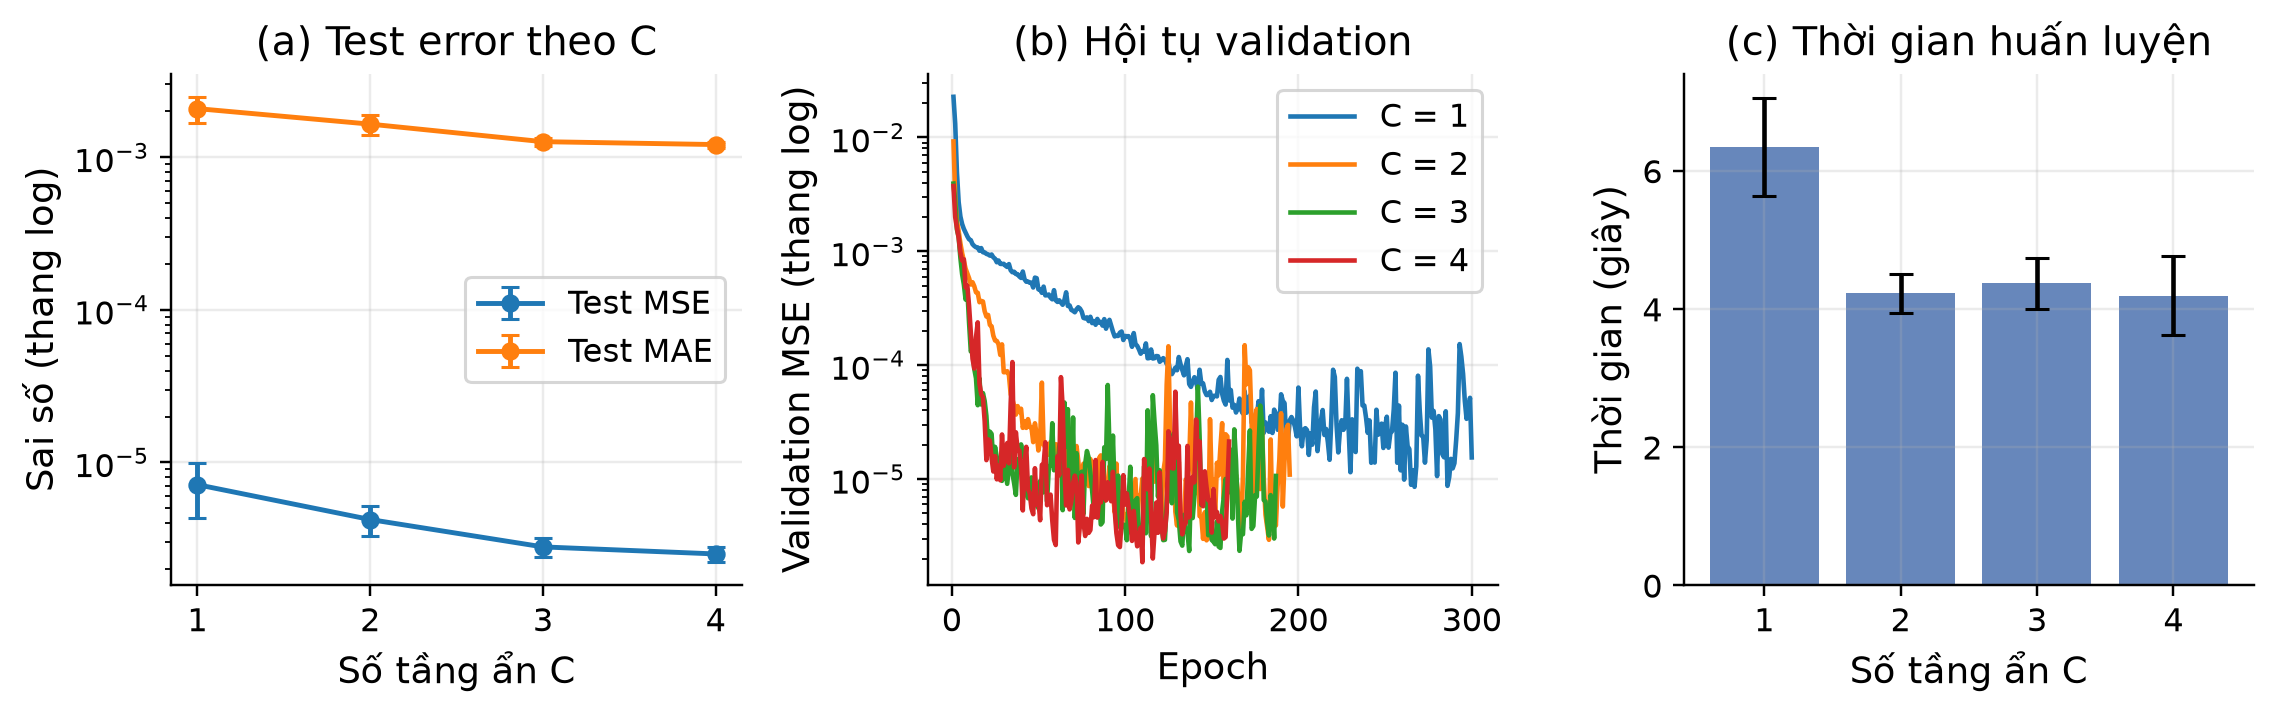
\includegraphics[width=1.0\textwidth]{figures/r10_expC.png}
\caption{Hình 10. Thực nghiệm C: (a) test error theo $C$; (b) hội tụ validation (seed 42); (c) thời gian huấn luyện trung bình.}
\end{figure}

\begin{figure}[h]
\centering
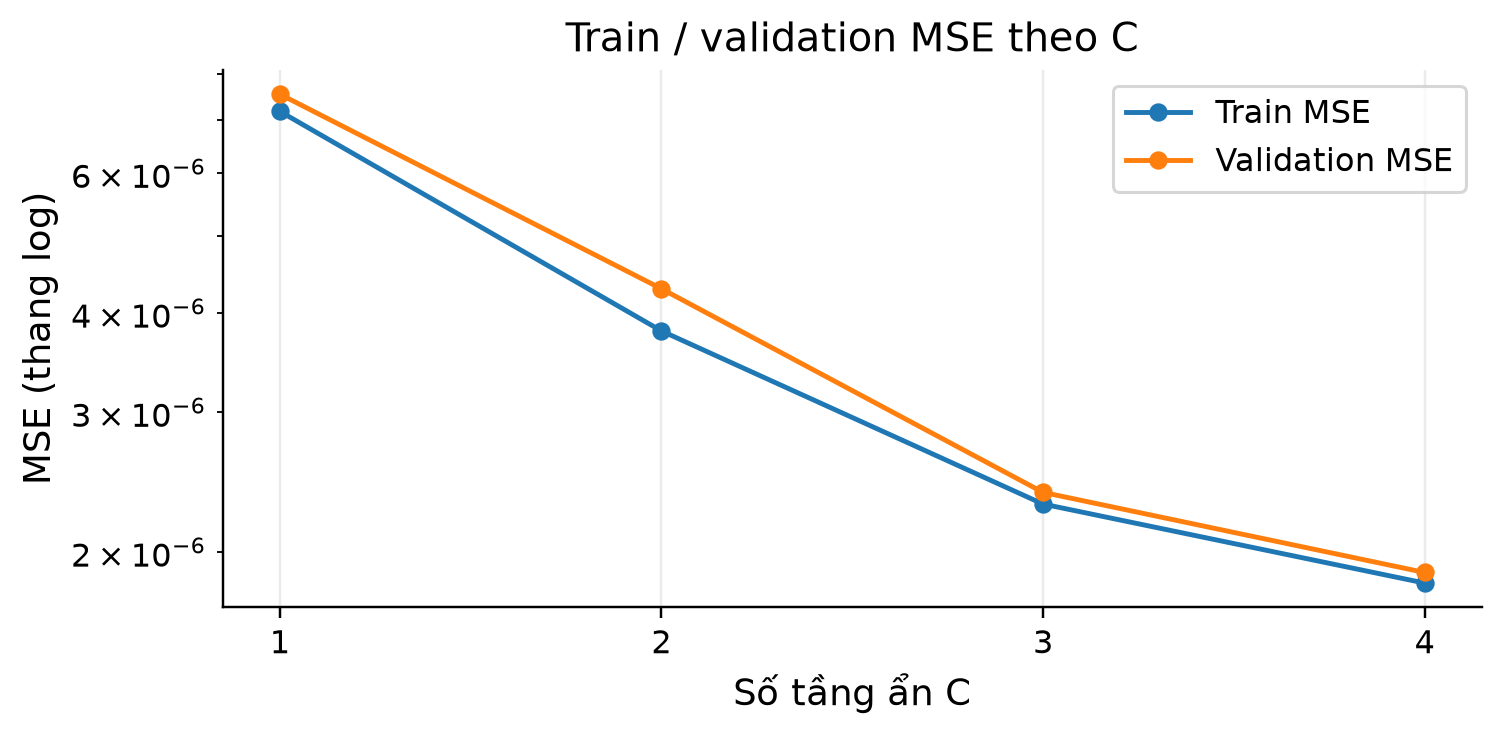
\includegraphics[width=0.8\textwidth]{figures/r11_expC_gap.png}
\caption{Hình 11. Thực nghiệm C: so sánh train và validation MSE theo số tầng ẩn.}
\end{figure}

Test MSE giảm từ $7.15\times10^{-6}$ ($C=1$) xuống $2.52\times10^{-6}$ ($C=4$), tức khoảng 2.8 lần, nhưng hiệu suất biên giảm nhanh: bước $C=1\to2$ cải thiện 1.7 lần, trong khi $C=3\to4$ chỉ còn 1.1 lần. Đường hội tụ trong Hình 10b cho thấy $C=1$ giảm chậm và bị nhiễu ở mức $10^{-5}$; $C=2$--$4$ hội tụ nhanh hơn, đạt vùng $10^{-6}$ sau khoảng 100--150 epoch. Mạng sâu hơn có thêm năng lực biểu diễn nên tối ưu hóa hiệu quả hơn ở giai đoạn đầu.

Thời gian trên mỗi epoch gần như không đổi (khoảng $0.0215$--$0.0229$ giây) vì mỗi lô chỉ có 64 mẫu và chi phí điều khiển của PyTorch chiếm phần lớn; chỉ khi $C=4$ mới nhích lên khoảng 6\%. Tổng thời gian huấn luyện không tăng đơn điệu vì bị chi phối bởi số epoch thực tế chạy: $C=1$ cần tới 294 epoch (6.35 giây) do hội tụ chậm, còn $C \ge 2$ dừng sớm hơn (183--200 epoch, 4.2--4.4 giây). Vì vậy, khi so sánh độ sâu cần đọc thời gian trên mỗi epoch thay vì chỉ nhìn tổng thời gian.

Không có dấu hiệu quá khớp: với $C=4$, train MSE $1.83\times10^{-6}$ và validation MSE $1.88\times10^{-6}$ gần như bằng nhau. Tăng độ sâu trong dải khảo sát chủ yếu cải thiện nhẹ độ chính xác chứ không làm mô hình ghi nhớ dữ liệu. Kết luận, $C=2$ là lựa chọn cân bằng giữa sai số và chi phí; $C=3$--$4$ chỉ đáng dùng nếu cần tối ưu thêm sai số rất nhỏ, còn $C=1$ vẫn khả thi nhưng cần nhiều epoch hơn.

\subsection{4.6. Chọn mô hình và đánh giá test cuối}

Mô hình được chọn chỉ dựa trên validation loss trung bình của tất cả cấu hình trong baseline và ba nhóm A/B/C. Bảng 7 trình bày các ứng viên tốt nhất theo từng nhóm. Cấu hình $A=1600$ với kiến trúc 2×64 có validation MSE thấp nhất ($1.14\times10^{-6}$), nhỉnh hơn $A=2000$ ($1.18\times10^{-6}$) nhưng khác biệt nằm trong sai số giữa các seed.

\begin{table}[h]
\centering
\caption{Bảng 7. Tổng hợp các cấu hình tốt nhất theo validation và kết quả test tương ứng.}
\begin{tabular}{|c|c|c|c|}
\hline
Cấu hình & Test MSE & Test MAE & Test RMSE \\
\hline
Baseline: $A=1000$, 2×64 & $3.26\times10^{-6}$ & $1.37\times10^{-3}$ & $1.80\times10^{-3}$ \\
\hline
A tốt nhất: $A=1600$, 2×64 & $1.41\times10^{-6}$ & $9.13\times10^{-4}$ & $1.17\times10^{-3}$ \\
\hline
B tốt nhất: $B=10$, 1 tầng ẩn & $8.20\times10^{-5}$ & $6.75\times10^{-3}$ & $8.86\times10^{-3}$ \\
\hline
C tốt nhất: $C=4$, $B=64$ & $2.52\times10^{-6}$ & $1.21\times10^{-3}$ & $1.58\times10^{-3}$ \\
\hline
Mô hình cuối: 2×64, 2000 mẫu & $1.09\times10^{-6}$ & $7.97\times10^{-4}$ & $1.04\times10^{-3}$ \\
\hline
\end{tabular}
\end{table}

Sau khi chọn cấu hình, mô hình được huấn luyện lại trên toàn bộ 2000 mẫu với ba seed; seed 44 có validation MSE thấp nhất ($1.02\times10^{-6}$) nên được lưu làm mô hình cuối. Trên tập test 100 mẫu, mô hình đạt MSE $1.09\times10^{-6}$, MAE $7.97\times10^{-4}$ và RMSE $1.04\times10^{-3}$. So với baseline, MSE giảm khoảng 3.0 lần và MAE giảm khoảng 1.7 lần, phù hợp với xu hướng của thực nghiệm A khi tăng số mẫu từ 1000 lên 2000.

Hình 12 và Hình 13 cho thấy dự đoán bám sát giá trị thật và bề mặt xấp xỉ gần như trùng với bề mặt thật. Hình 14 cho thấy phần dư tập trung quanh 0, không có xu hướng hệ thống; một vài mẫu ở đuôi có sai số lớn hơn nhưng đóng góp vào MSE không đáng kể vì $y$ ở đó rất nhỏ.

\begin{figure}[h]
\centering
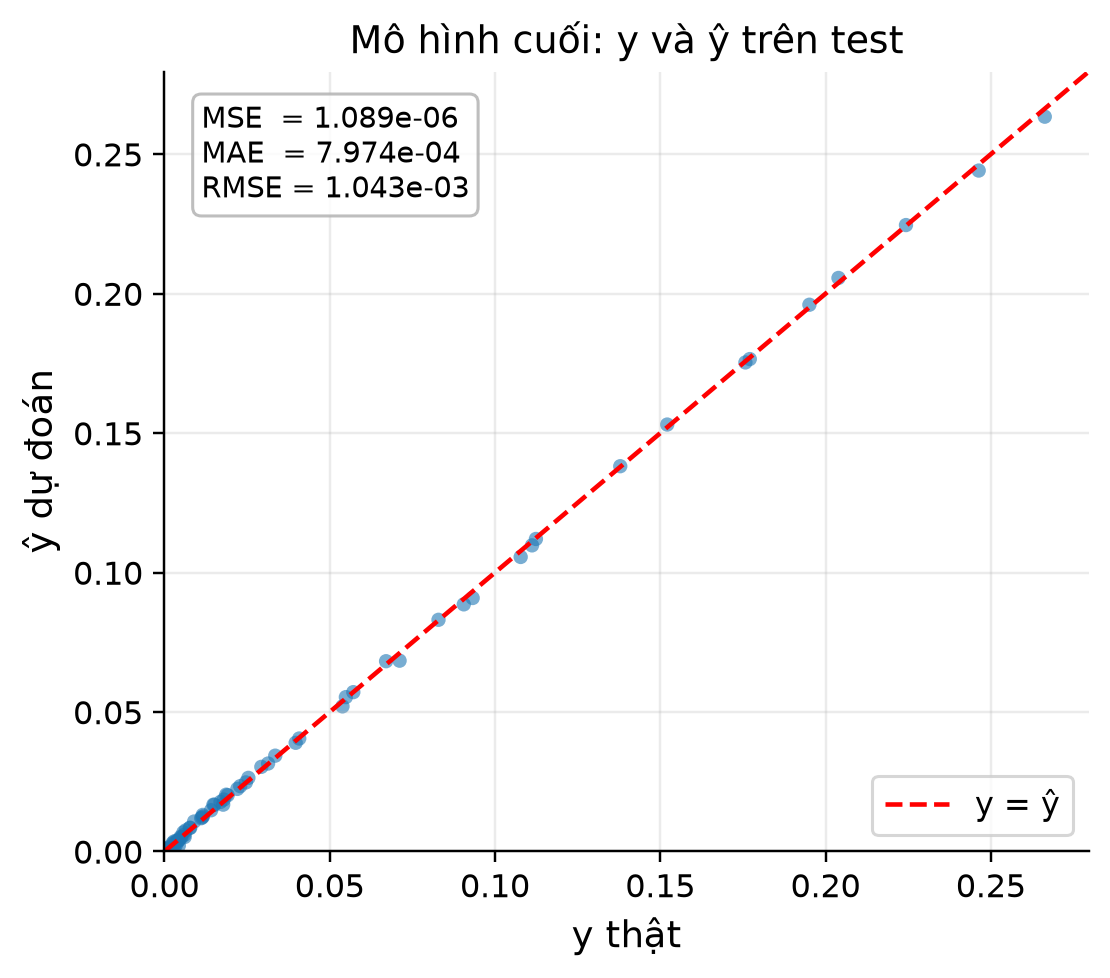
\includegraphics[width=0.62\textwidth]{figures/r12_final_yhat.png}
\caption{Hình 12. Mô hình cuối: so sánh $y$ thật và $\hat{y}$ trên tập test.}
\end{figure}

\begin{figure}[h]
\centering
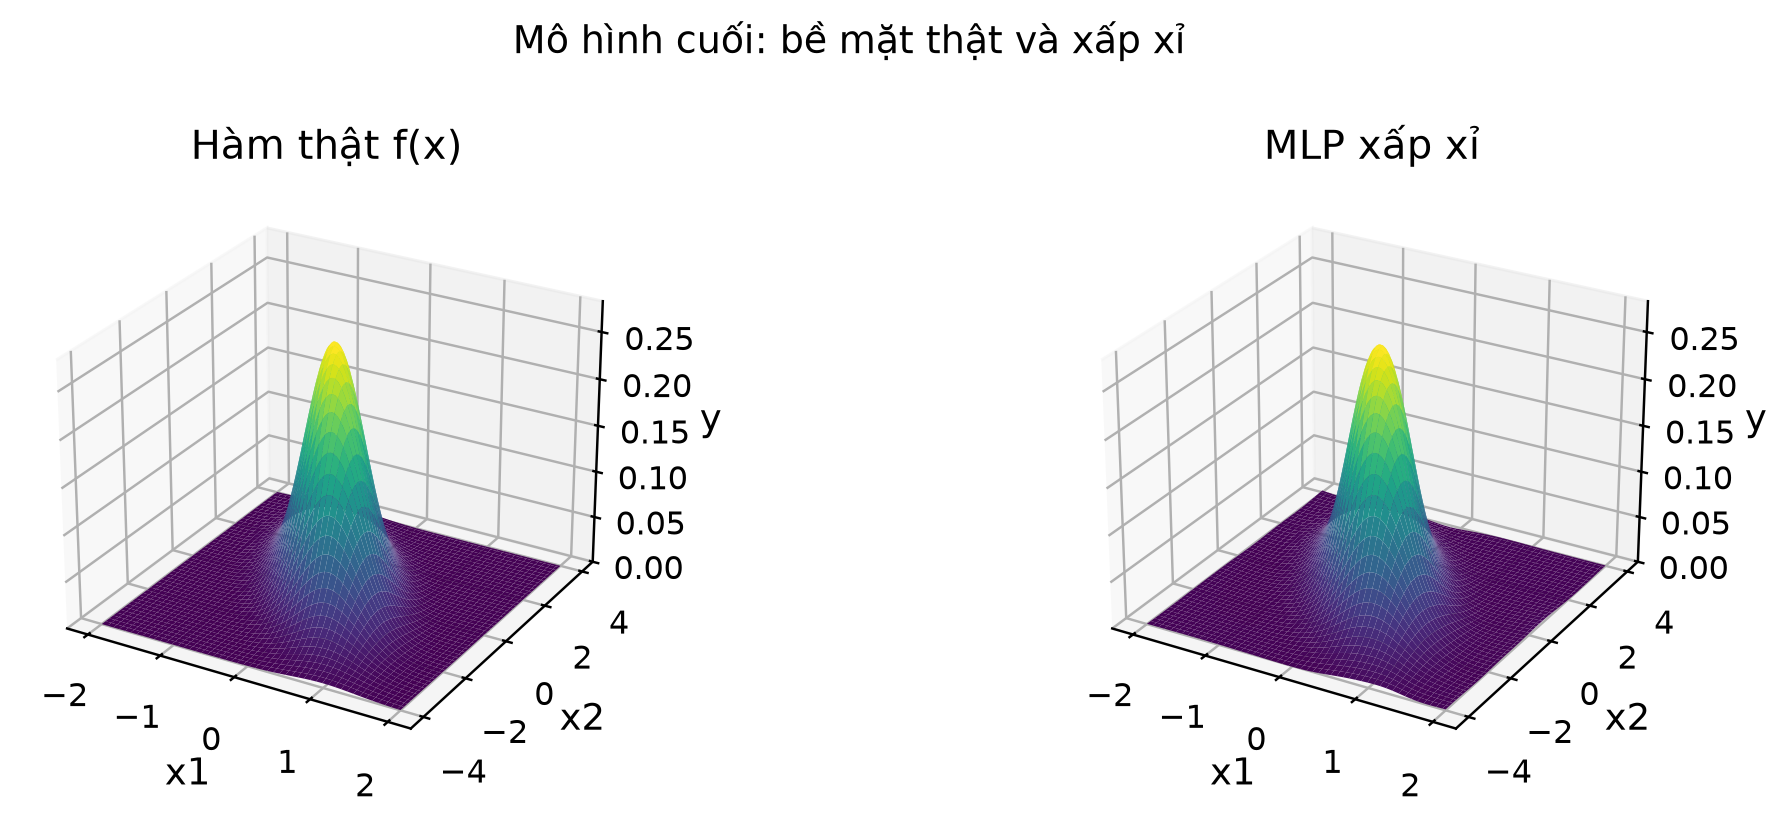
\includegraphics[width=0.95\textwidth]{figures/r13_final_surface.png}
\caption{Hình 13. Mô hình cuối: so sánh bề mặt hàm thật và bề mặt xấp xỉ.}
\end{figure}

\begin{figure}[h]
\centering
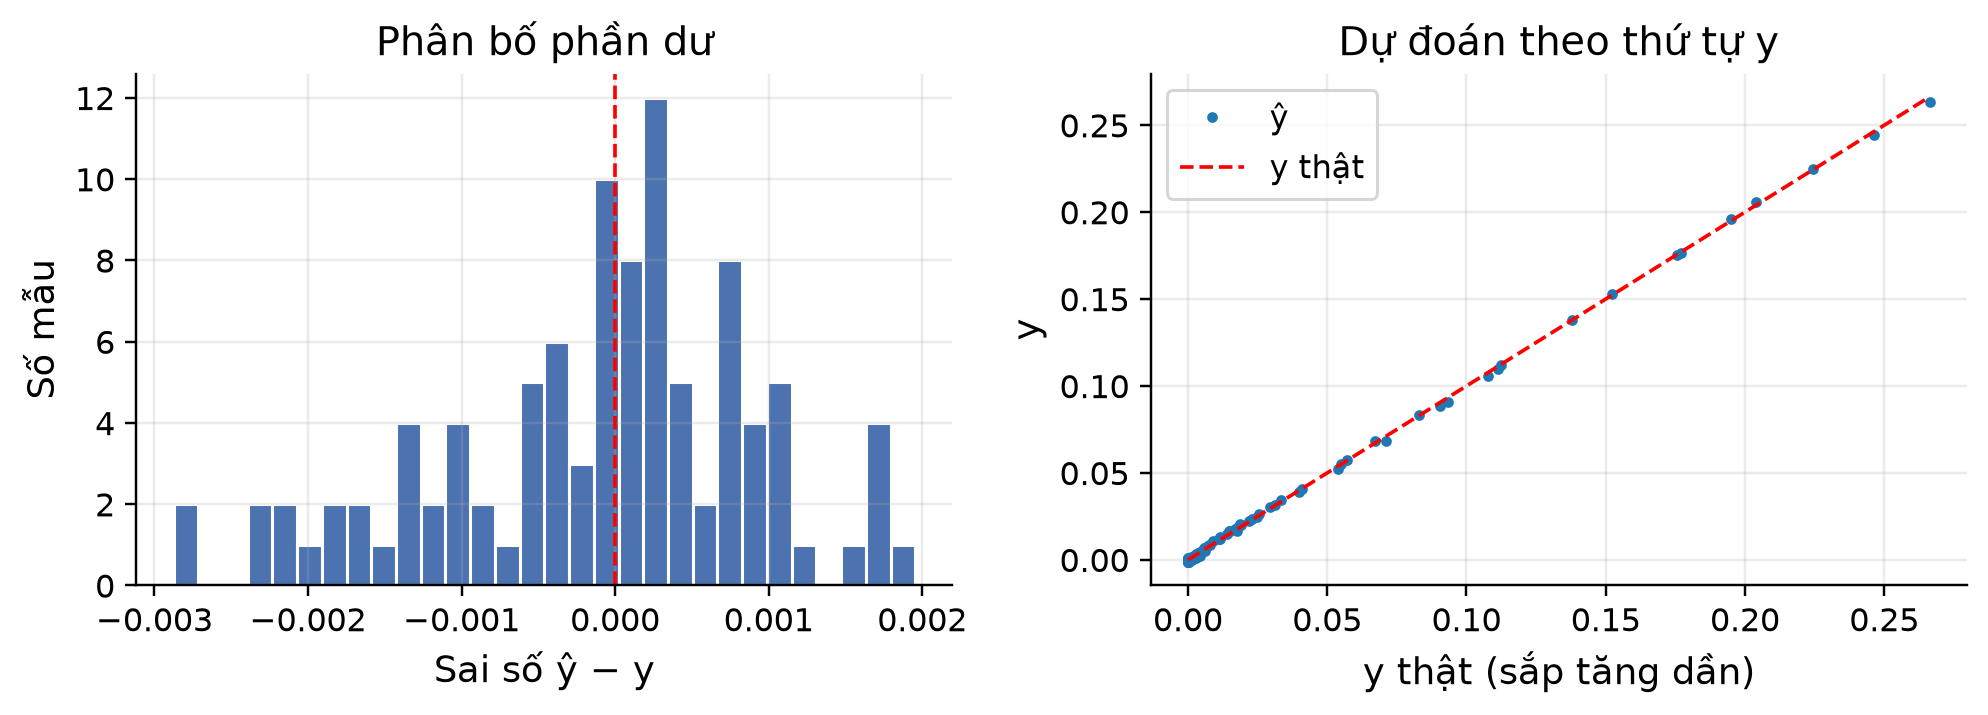
\includegraphics[width=0.9\textwidth]{figures/r14_final_residuals.png}
\caption{Hình 14. Mô hình cuối: phân bố phần dư trên test và dự đoán theo thứ tự $y$ thật.}
\end{figure}

\section{5. Thảo luận}

\subsection{5.1. Xu hướng chính}

Ba thực nghiệm cho thấy bức tranh nhất quán. Về quy mô dữ liệu, sai số giảm mạnh khi tăng $A$ nhưng hiệu suất biên giảm sau khoảng 1000--1200 mẫu. Về độ rộng, mạng một tầng ẩn cần ít nhất khoảng bốn nơ-ron để vượt qua vùng dự đoán trung bình, và sai số tiếp tục giảm đến $B=10$ nhưng chưa bão hòa. Về độ sâu, hai tầng ẩn đã đủ cho bài toán; tăng lên ba hoặc bốn tầng chỉ cải thiện nhẹ.

Có thể giải thích các xu hướng này bằng độ phức tạp của hàm mục tiêu. Hàm Gaussian hai chiều là hàm trơn, bị chi phối bởi một đỉnh hẹp và một hướng tương quan. Một mạng đủ rộng và đủ sâu có thể xấp xỉ hàm này với sai số rất nhỏ khi dữ liệu che phủ vùng đỉnh. Khi $A$ tăng, mật độ mẫu quanh đỉnh tăng, giúp mô hình học được độ cong và hướng nghiêng chính xác hơn. Khi $B$ tăng, mạng có thêm "cơ sở" để biểu diễn hàm; khi $C$ tăng, mạng có thể tổ hợp các đặc trưng phi tuyến, nhưng với hàm đơn giản này lợi ích của tầng sâu thêm là hạn chế.

\subsection{5.2. Các trường hợp không như kỳ vọng}

Có bốn điểm cần diễn giải cẩn thận. Thứ nhất, trong thực nghiệm A, sai số không giảm đơn điệu: $A=1000$ có test MSE cao hơn $A=800$, và $A=1800$ cao hơn $A=1600$. Vì độ lệch chuẩn giữa các seed ở các cấu hình này chồng lấn đáng kể, không nên coi đây là bằng chứng rằng thêm dữ liệu làm mô hình tệ đi. Nguyên nhân khả dĩ là khởi tạo mạng và thời điểm early stopping khác nhau, cùng với việc tập test chỉ có 100 mẫu nên bản thân ước lượng sai số đã có dao động lấy mẫu.

Thứ hai, trong thực nghiệm B, $B=9$ và $B=10$ có test MSE gần như bằng nhau ($8.35\times10^{-5}$ và $8.20\times10^{-5}$) trong khi độ lệch chuẩn của $B=10$ lớn hơn. Không thể kết luận $B=10$ tốt hơn $B=9$ một cách chắc chắn. Điểm chắc chắn là cả hai đều tốt hơn rõ rệt $B \le 8$, và cả hai vẫn chưa đạt tới vùng bão hòa vì epoch tốt nhất gần sát 300.

Thứ ba, tổng thời gian huấn luyện trong thực nghiệm C không tăng theo $C$ do early stopping. Đây là hiện tượng bình thường khi so sánh các cấu hình có số epoch chạy khác nhau; đại lượng phản ánh chi phí tính toán tốt hơn là thời gian trên mỗi epoch. Thời gian này tăng rất nhẹ từ $C=1$ đến $C=4$ vì kích thước lô nhỏ và chi phí điều khiển chiếm ưu thế.

Thứ tư, ở một số lượt chạy, validation MSE thấp hơn train MSE. Điều này không mâu thuẫn với lý thuyết: validation là một tập mẫu khác, có thể "dễ" hơn ở vùng đuôi; ngoài ra trọng số được chọn theo validation nên có thiên lệch nhẹ theo hướng làm đẹp chỉ số này. Với sai số ở mức $10^{-6}$, chênh lệch vài phần trăm không có ý nghĩa thực tiễn.

\subsection{5.3. Lựa chọn mô hình và đánh đổi}

Mô hình cuối dùng 2 tầng ẩn 64 nơ-ron và 2000 mẫu. Đây là lựa chọn cân bằng: sai số test thấp nhất trong các cấu hình đã khảo sát, thời gian huấn luyện dưới 10 giây trên CPU, số tham số 4417 nên dễ lưu trữ và triển khai. Việc tăng thêm độ sâu hoặc độ rộng có thể giảm sai số thêm nhưng lợi ích rất nhỏ so với chi phí và rủi ro tối ưu (dao động giữa các seed).

Một điểm cần nhấn mạnh là kết quả test cuối không được dùng để chọn mô hình. Nếu dùng test để chọn giữa các cấu hình, con số báo cáo sẽ lạc quan hơn thực tế. Trong báo cáo này, validation là tiêu chí duy nhất cho checkpoint, early stopping và lựa chọn cuối; test chỉ được đánh giá một lần sau khi đã chốt cấu hình.

\subsection{5.4. Hạn chế}

Báo cáo có một số hạn chế. Thứ nhất, các thí nghiệm chỉ chạy trên CPU với mạng nhỏ, chưa khảo sát learning-rate schedule, weight decay, BatchNorm, residual connection hay các hàm kích hoạt khác như ReLU, GELU, SiLU. Thứ hai, dữ liệu không có nhiễu và hàm mục tiêu trơn nên kết quả khá lạc quan; với dữ liệu thực cần thêm nhiễu, kiểm tra chéo $k$-fold và phân tích độ bất định. Thứ ba, tập test chỉ có 100 mẫu, đủ để so sánh tương đối nhưng chưa đủ để ước lượng sai số với khoảng tin cậy hẹp. Thứ tư, dải $B$ bị giới hạn ở 1--10 theo yêu cầu nên chưa quan sát được vùng quá khớp; để thấy hiện tượng này cần mở rộng $B$ lên hàng chục hoặc hàng trăm và giảm $A$.

\subsection{5.5. Hướng cải tiến}

Có thể mở rộng theo bốn hướng. Một là khảo sát thêm learning rate, batch size và activation để tìm cấu hình tốt hơn với cùng ngân sách. Hai là thêm nhiễu Gaussian vào nhãn và đánh giá độ bền của mô hình. Ba là dùng $k$-fold cross-validation thay cho một tập validation cố định, đặc biệt khi $A$ nhỏ. Bốn là thử các kiến trúc hiện đại hơn như Fourier features hoặc mạng residual để cải thiện xấp xỉ vùng đỉnh nhọn.

\section{6. Kết luận}

Báo cáo đã xây dựng thành công mô hình MLP bằng PyTorch để xấp xỉ hàm mật độ Gaussian hai chiều, với quy trình dữ liệu, huấn luyện và đánh giá có thể tái lập. Ba nhóm thực nghiệm cho thấy: (i) số mẫu huấn luyện là yếu tố ảnh hưởng mạnh nhất trong dải khảo sát, giúp giảm MSE khoảng 19 lần từ 200 lên 2000 mẫu; (ii) độ rộng tầng ẩn có ngưỡng tối thiểu rõ rệt, dưới bốn nơ-ron mô hình gần như chỉ dự đoán giá trị trung bình; (iii) độ sâu từ hai tầng trở lên mang lại cải thiện nhỏ và nhanh chóng bão hòa.

Mô hình cuối cùng (2 tầng ẩn 64 nơ-ron, huấn luyện trên 2000 mẫu) đạt MSE $1.09\times10^{-6}$, MAE $7.97\times10^{-4}$ và RMSE $1.04\times10^{-3}$ trên tập test 100 mẫu, tốt hơn baseline khoảng 3 lần về MSE. Kết quả này cho thấy với một hàm trơn, hai chiều và dữ liệu được lấy mẫu hợp lý, một mạng MLP nhỏ đã đủ để đạt sai số rất thấp; yếu tố quyết định không phải là mô hình quá lớn mà là đủ dữ liệu, đủ năng lực tối thiểu và quy trình đánh giá đúng.

\section*{Tài liệu tham khảo}

\begin{enumerate}
\item I. Goodfellow, Y. Bengio, A. Courville. \textit{Deep Learning}. MIT Press, 2016.
\item C. M. Bishop. \textit{Pattern Recognition and Machine Learning}. Springer, 2006.
\item A. Paszke et al. \textit{PyTorch: An Imperative Style, High-Performance Deep Learning Library}. Advances in Neural Information Processing Systems (NeurIPS), 2019.
\item D. P. Kingma, J. Ba. \textit{Adam: A Method for Stochastic Optimization}. International Conference on Learning Representations (ICLR), 2015.
\item L. Prechelt. \textit{Early Stopping -- But When?} Neural Networks: Tricks of the Trade, Springer, 1998.
\item PyTorch Documentation. \texttt{https://pytorch.org/docs/stable/index.html}, truy cập tháng 10/2026.
\end{enumerate}

\section*{Phụ lục A. Cấu trúc mã nguồn và tái lập}

Mã nguồn được đặt trong thư mục \texttt{BTL01/} với cấu trúc:

\begin{itemize}
\item \texttt{BTL01\_MLP\_Gaussian.ipynb}: notebook chính, chia mục 0--9.
\item \texttt{requirements.txt}: danh sách thư viện.
\item \texttt{README.md}: hướng dẫn chạy và mô tả đầu ra.
\item \texttt{outputs/data/}: \texttt{train\_pool.csv}, \texttt{validation.csv}, \texttt{test.csv}.
\item \texttt{outputs/logs/}: \texttt{results\_A.csv}, \texttt{results\_B.csv}, \texttt{results\_C.csv}, \texttt{results\_baseline.csv}, \texttt{summary\_all.csv}, \texttt{final\_test\_results.csv} và các file lịch sử loss.
\item \texttt{outputs/figures/}: 14 hình được dùng trong báo cáo.
\item \texttt{outputs/models/runs/}: checkpoint từng lượt chạy; \texttt{outputs/models/best\_model.pt}: mô hình cuối.
\end{itemize}

Để tái lập, cài đặt môi trường bằng \texttt{pip install -r requirements.txt}, sau đó chạy toàn bộ notebook từ thư mục \texttt{BTL01/}. Thời gian chạy trên CPU khoảng 10--15 phút. Toàn bộ seed, cấu hình và đường dẫn được khai báo trong notebook.

\end{document}
